\subsubsection{UI-Testservice}

Das UI-Testservice ist die Dienststelle, die für die Durchführung
von UI-Tests verantwortlich ist. Es besteht im Wesentlichen aus
vier Containern:

\begin{itemize}
    \setlength\itemsep{1em}

    \item[] \textbf{Selenium-Hub, Chrome- und Firefox-RemoteWebDriver}:
    Der Selenium Hub ist ein Server, der die Zugriffsanfragen vom 
    WebDriver-Client entgegennimmt und die JSON-Testbefehle an die 
    entfernten (remote) Driver weiterleitet. Er nimmt die Befehle vom 
    Client entgegen und führt sie parallel auf den verschiedenen 
    remote Driver aus. Dies ermöglicht die Verwendung der 
    RemoteWebDriver Chrome und Firefox, die direkt mit dem
    Selenium-Hub verbunden sind. Der Tester kann also wählen,
    welchen Browser er für die Ausführung seiner Tests verwenden
    möchte. Es ist jedoch wichtig, darauf hinzuweisen, dass die 
    Container, die die RemoteWebDriver enthalten, so konfiguriert 
    sind, dass sie mit der neuesten Version des Browsers ausgeführt 
    werden, die bei jedem Docker Image Build automatisch 
    heruntergeladen wird.

    \item[] \textbf{UI-Test}: Dieser Container enthält die UI-Tests
    und ist dafür zuständig, diese automatisch mithilfe eines
    Maven-Skripts auszuführen. Wenn die Tests im Remote-Modus
    konfiguriert sind, verbindet sich der Container mit dem
    Selenium-Hub, um Zugriff auf den verfügbaren RemoteWebDriver
    zu erhalten.
\end{itemize}

\begin{figure}[H]
    \centering
    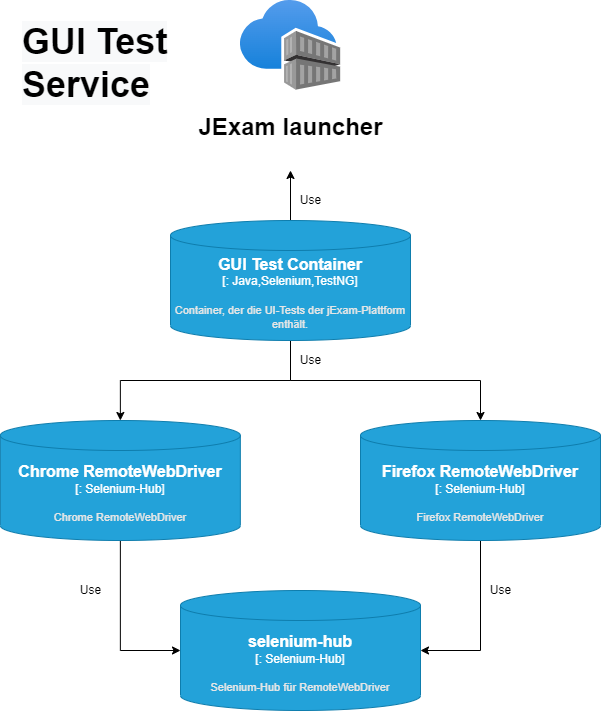
\includegraphics[scale=0.6]{images/gui.drawio}
    \caption{JExam UI Testservice} \label{fig:ui}
\end{figure}